\documentclass[aspectratio=1610,14pt]{beamer}

\usepackage[utf8]{inputenc}
\usepackage{graphicx}
\usepackage{url}
\usepackage{minted}

\graphicspath{{images/}}
\usetheme{csctraining}
\usemintedstyle{solarized-dark}

\newcommand{\link}[1]{\alert{\url{#1}}}
\newcommand{\vitem}{\vfill\item}

\title{Machine Learning \\at CSC}
\subtitle{June 3, 2020\\[2mm]
  Mats Sjöberg -- mats.sjoberg@csc.fi}

\begin{document}

\begin{frame}{Overview}
  \tableofcontents
\end{frame}

\section{What CSC service to use?}

% TODO try with larger image and step-by-step display of each service
% with text apparing and disappearing - circle around place in picture

\begin{frame}{What CSC service to use?}
  \begin{itemize}
  \item CSC's supercomputer \alert{Puhti}
    \begin{itemize}
    \item<2-> Cluster with GPU-accelerated nodes
    \item<2-> Multi-user environment
    \end{itemize}
  \item Virtual server on \alert{Pouta}
    \begin{itemize}
    \item<3-> Your ``own'' server
    \item<3-> Less powerful than Puhti
    \end{itemize}
  \item Container cloud \alert{Rahti}
    \begin{itemize}
    \item<4-> Easy to run containers
    \item<4-> No GPUs \textbf{yet}
    \end{itemize}
  \end{itemize}
  \vspace{-5mm}
  \begin{flushright}
  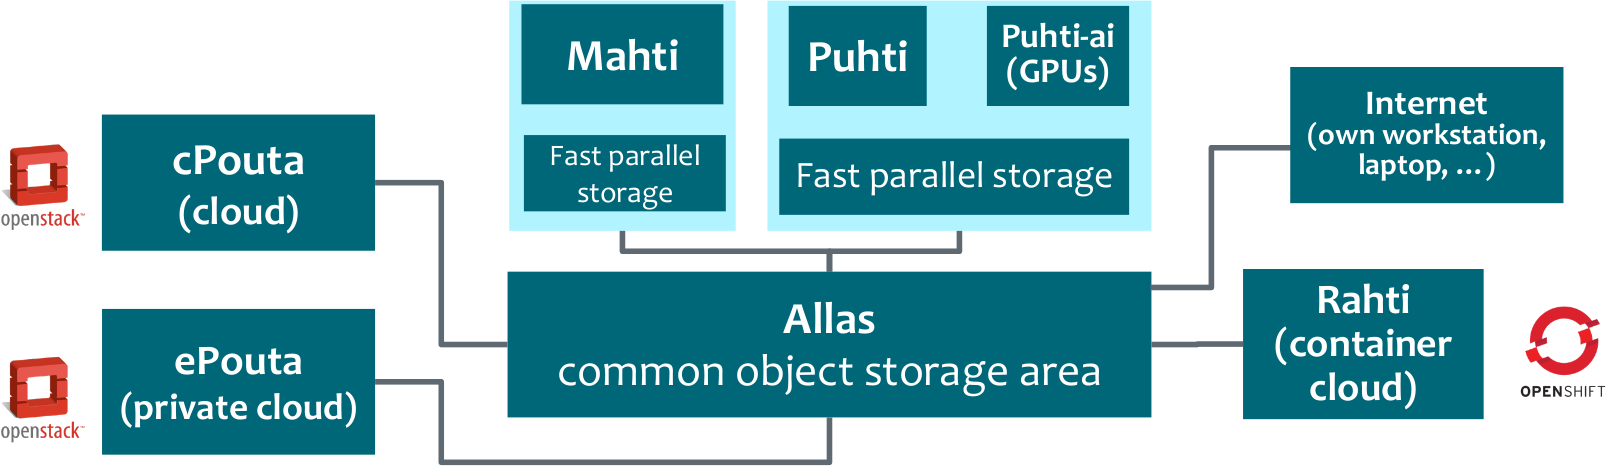
\includegraphics[width=0.9\textwidth]{csc-services}  
  \end{flushright}
\end{frame}

\section{Puhti supercomputer}

\begin{frame}{Puhti supercomputer}
  \begin{columns}
    \begin{column}{0.76\linewidth}
      \begin{minipage}[c][0.6\textheight][s]{\columnwidth}
      \begin{itemize}
        \item \emph{Puhti-AI}, cluster with 80 nodes with \mbox{4 GPUs}
        each $\rightarrow$ 320 GPUs in total
        \vitem Latest generation Nvidia V100 GPUs (Volta) with 32 GB of memory
        \vitem Fast network: 2 $\times$ 100 Gbps links to each node
        \vitem Each node has a fast 3.2 TB local NVME disk
      \end{itemize}
      \vfill
      \end{minipage}
    \end{column}
    %% 
    \begin{column}{0.24\linewidth}
      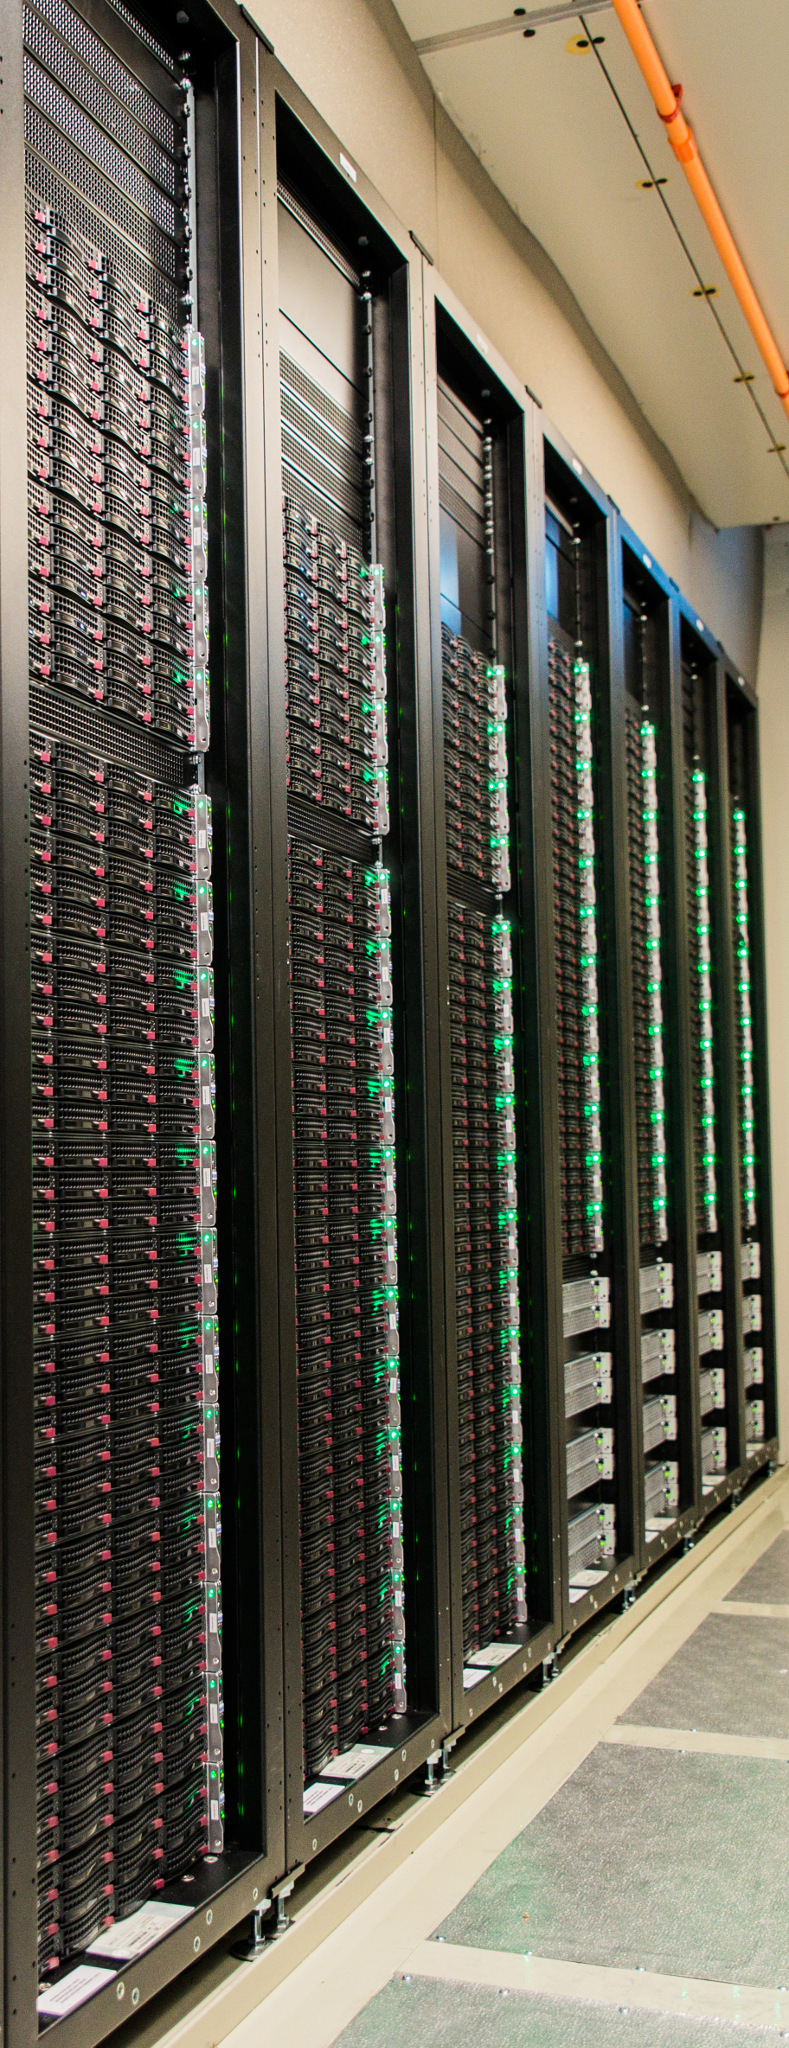
\includegraphics[height=0.8\textheight]{puhti-long}
    \end{column}
  \end{columns}
\end{frame}

\begin{frame}{Getting access to Puhti}
  \link{https://docs.csc.fi/computing/overview/}

  \vspace{1em}

  To use Puhti you need to:
  \begin{itemize}
  \item Have a CSC account
  \item Be member of a CSC project, either by
    \begin{itemize}
    \item creating a new project, or
    \item joining an existing project (ask the PI to add you!)
    \end{itemize}
  \item Finally, the project needs to have Puhti access
  \end{itemize}

  \vspace{1em}

  $\rightarrow$ \quad MyCSC portal: \link{https://my.csc.fi/}

\end{frame}

\begin{frame}[fragile]{Accessing Puhti}
  \begin{itemize}
  \item Using an ssh client such as OpenSSH or PuTTY
  \item Basic Linux skills are required!
  \item More info: \link{https://docs.csc.fi/computing/connecting/}
  \end{itemize}

  \vspace{1em}

\begin{verbatim}
ssh <csc_username>@puhti.csc.fi
\end{verbatim}

\begin{verbatim}
ssh <csc_username>@puhti-login2.csc.fi
\end{verbatim}

\end{frame}

\begin{frame}{Supported frameworks}
  We currently support:
  \begin{itemize}
  \item \alert{Python Data} -- collection of Python libraries for data
    analytics and machine learning
  \item \alert{TensorFlow} -- deep learning library for Python
  \item \alert{PyTorch} -- machine learning framework for Python
  \item \alert{MXNet} -- deep learning library for Python
  \item \alert{RAPIDS} -- suite of libraries for data analytics and
    machine learning on GPUs
  \end{itemize}

  {\small \link{https://docs.csc.fi/apps/\#data-analytics-and-machine-learning}}
\end{frame}

\begin{frame}[fragile]{Example: TensorFlow}
  \begin{itemize}
  \vitem First check the application page for instructions:
    \link{https://docs.csc.fi/apps/tensorflow/}
  \vitem Load the default version:
\begin{verbatim}
module load tensorflow
\end{verbatim}
  \vitem or specific version:
\begin{verbatim}
module load tensorflow/2.0.0
\end{verbatim}
  \vitem \alert{Note:} some modules are \emph{Singularity-based}!
\end{itemize}
\vfill
\end{frame}

\begin{frame}[fragile]{What if some package is missing?}
  If you are using our module, but a trivial package is missing \ldots
  \begin{itemize}
  \vitem install it yourself, e.g.,
\begin{verbatim}
pip install --user <packagename>
\end{verbatim}
  \vitem \ldots or if it might be generally useful, send an email to \alert{\tt
      servicedesk@csc.fi} -- we can install it for you!
  \end{itemize}
  \vfill
  
\end{frame}

\begin{frame}[fragile]{What if some package is missing?}
  If you need a specific setup, and our modules are not right for you \ldots
  \begin{itemize}
  \vitem use a virtualenv:
\begin{verbatim}
python3 -m venv myenv
source myenv/bin/activate
pip install ...
\end{verbatim}
    
  \vitem use conda: {\small \link{https://docs.csc.fi/support/tutorials/conda/}}
  \vitem use singularity containers: {\small \link{https://docs.csc.fi/computing/containers/run-existing/}}
    
  \vitem or if generally useful, send an email to \alert{\tt
      servicedesk@csc.fi}
  \end{itemize}
  
\end{frame}

\begin{frame}{Running a job on Puhti}
  \alert{Don't run heavy computing jobs in the login nodes!}
  \vspace{2mm}
  \begin{itemize}
  \item Puhti uses the \emph{Slurm} batch job system
  \item Jobs do not run instantly but are put in a \emph{queue}
  \item Resources (runtime, memory, number of cores) need to be specified
  \end{itemize}

  \vspace{-4mm}
  \begin{center}
    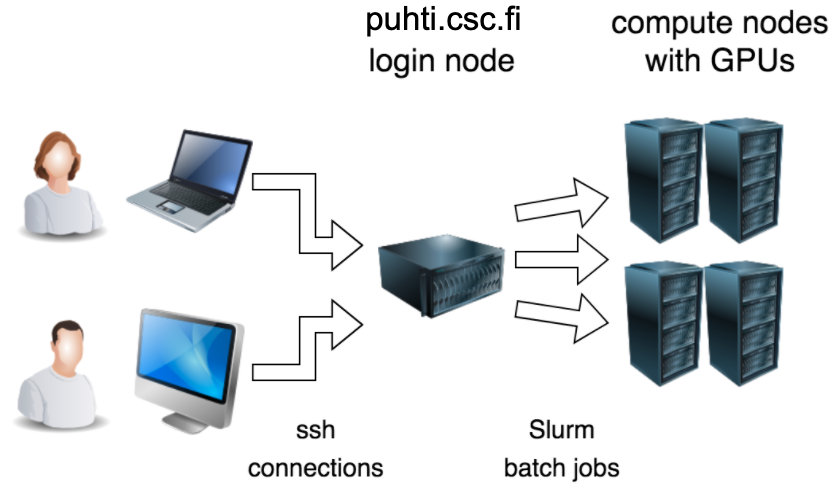
\includegraphics[width=0.55\textwidth]{slurm1.png}    
  \end{center}
\end{frame}

\begin{frame}{Running a job on Puhti}
  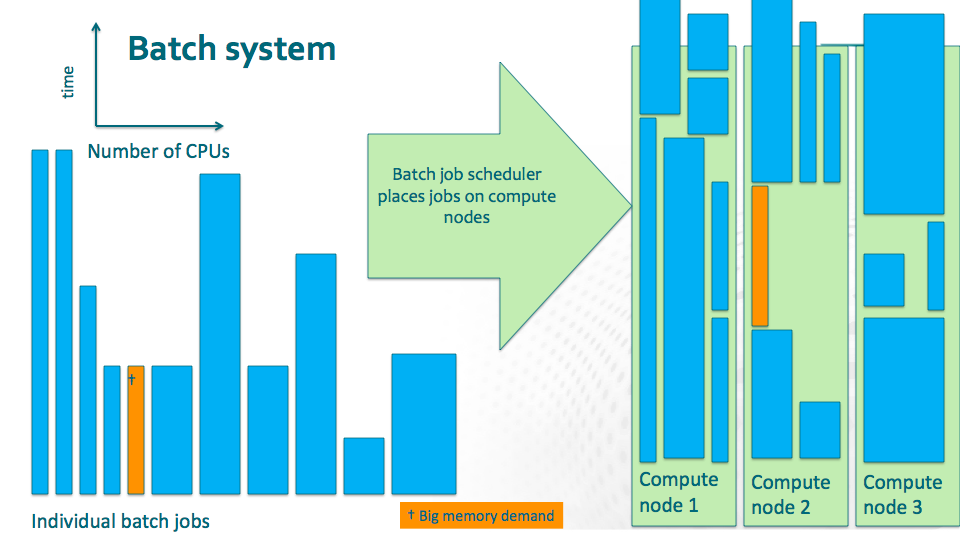
\includegraphics[width=\textwidth]{slurm2.png}
\end{frame}

\begin{frame}[fragile]{Running a job on Puhti}

  Create a job script, for example {\tt run.sh}:
  
\definecolor{bg}{rgb}{0.95,0.95,0.95}
\definecolor{hl}{rgb}{0.95,0.95,0.05}
\begin{minted}[bgcolor=bg,fontsize=\small,highlightlines={3,8},highlightcolor=hl]{bash}
#!/bin/bash
#SBATCH --account=<project>
#SBATCH --partition=gpu
#SBATCH --ntasks=1
#SBATCH --cpus-per-task=10
#SBATCH --mem=64G
#SBATCH --time=1:00:00
#SBATCH --gres=gpu:v100:1

module load tensorflow/2.0.0
srun python3 myprog.py <options>
\end{minted}

{\small \link{https://docs.csc.fi/computing/running/creating-job-scripts/}}
\end{frame}

\begin{frame}[fragile]{Running a job on Puhti}
  Submit the job:
\begin{verbatim}
sbatch run.sh
\end{verbatim}
  \vfill
  
  Check the queue:
\begin{verbatim}
squeue -l -u $USER
\end{verbatim}
  \vfill
  
  Cancel a job:
\begin{verbatim}
scancel <jobid>
\end{verbatim}

  {\small \link{https://docs.csc.fi/computing/running/submitting-jobs/}}
\end{frame}

\section{Data storage}

\begin{frame}{Data storage on Puhti}
  
  {\footnotesize
    \begin{tabular}{lllrrl}
             & Owner    & Path                      & Capacity & Number of files & Cleaning \\
    \hline
    home     & Personal & {\tt /users/<user-name>}  & 10 GiB   & 100 000 files   & No \\
    projappl & Project  & {\tt /projappl/<project>} & 50 GiB   & 100 000 files   & No \\
    scratch  & Project  & {\tt /scratch/<project>}  & 1 TiB    & 1 000 000 files & Yes - 90 days \\
    \end{tabular}
  }
  \vspace{1em}

  \begin{itemize}
  \item Disk space and \emph{number of files} are limited on Puhti!
    \begin{itemize}
    \item Reason: we want to ensure that the shared (Lustre) filesystem
      works efficiently for everyone!
    \end{itemize}
  \item Data quotas can be increased via MyCSC!
  \end{itemize}

  % \vspace{1em}
  
  {\small \link{https://docs.csc.fi/computing/disk/}}
\end{frame}

\section{GPU utilization}

\section{Multi-GPU and multi-node jobs}

\section{Singularity containers}

\end{document}

%%% Local Variables: 
%%% TeX-command-extra-options: "-shell-escape"
%%% End:
